%% ======================================================================
%% ExoGame: Plataforma Gamificada de Perguntas e Respostas sobre
%% Exoplanetas 
%% 

\documentclass[
	12pt,
	openany,
	oneside,
	a4paper,
	english,
	brazil
]{abntex2}

% ---
% Pacotes básicos
% ---
\usepackage{lmodern}
\usepackage[T1]{fontenc}
\usepackage[utf8]{inputenc}
\usepackage{indentfirst}
\usepackage{color}
\usepackage{graphicx}
\usepackage{microtype}
\usepackage{listings}
\usepackage{xcolor}
\usepackage{tikz}
\usepackage{booktabs}
\usepackage{multirow}
\usepackage{longtable}
\usepackage{tabularx}
\usepackage{amsmath}

% TikZ libraries
\usetikzlibrary{shapes.geometric, arrows.meta, positioning, fit, calc, backgrounds}

% ---
% Configuração de listings para código-fonte
% ---
\definecolor{codebg}{RGB}{245,245,245}
\definecolor{codegreen}{RGB}{0,128,0}
\definecolor{codegray}{RGB}{128,128,128}
\definecolor{codepurple}{RGB}{128,0,128}
\definecolor{codeblue}{RGB}{0,0,200}

\lstdefinestyle{codestyle}{
  backgroundcolor=\color{codebg},
  commentstyle=\color{codegreen}\itshape,
  keywordstyle=\color{codeblue}\bfseries,
  stringstyle=\color{codepurple},
  basicstyle=\ttfamily\footnotesize,
  breakatwhitespace=false,
  breaklines=true,
  captionpos=b,
  keepspaces=true,
  numbers=left,
  numbersep=5pt,
  numberstyle=\tiny\color{codegray},
  showspaces=false,
  showstringspaces=false,
  showtabs=false,
  tabsize=2,
  frame=single,
  rulecolor=\color{codegray},
  language=Ruby, % sintaxe próxima ao Elixir
  morekeywords={defmodule, def, defp, do, end, case, receive, when, after,
    fn, true, false, nil, and, or, not, in, use, alias, require, import,
    send, spawn, self, exit, raise, rescue, with, for, if, else, unless,
    cond, try, catch, throw, super, quote, unquote, struct, module,
    @moduledoc, @doc, @spec, @type, @callback, @behaviour, @derive,
    GenServer, Supervisor, Application, Phoenix, Repo, Ecto,
    handle_call, handle_cast, handle_info, init, start_link, terminate,
    defstruct, defprotocol, defimpl, defmacro, defmacrop,
    join, leave, handle_in, broadcast, push, reply,
    const, let, export, import, from, interface, type, async, await},
  morestring=[b]',
  morestring=[b]",
  literate={á}{{\'a}}1 {é}{{\'e}}1 {í}{{\'i}}1 {ó}{{\'o}}1 {ú}{{\'u}}1
           {ã}{{\~a}}1 {õ}{{\~o}}1 {ç}{{\c{c}}}1 {Ç}{{\c{C}}}1
           {â}{{\^a}}1 {ê}{{\^e}}1 {ô}{{\^o}}1
}

\lstset{style=codestyle}

% ---
% Pacotes de citações
% ---
\usepackage[brazilian,hyperpageref]{backref}
\usepackage[alf]{abntex2cite}

% ---
% Configurações do pacote backref
% ---
\renewcommand{\backrefpagesname}{Citado na(s) página(s):~}
\renewcommand{\backref}{}
\renewcommand*{\backrefalt}[4]{%
	\ifcase #1
		Nenhuma citação no texto.%
	\or
		Citado na página #2.%
	\else
		Citado #1 vezes nas páginas #2.%
	\fi}

% ---
% Informações de dados para CAPA e FOLHA DE ROSTO
% ---
\titulo{ExoGame: Plataforma Gamificada de Perguntas e Respostas sobre Exoplanetas}
\autor{REINAN BEZERRA DA SILVA SANTOS}
\local{JUAZEIRO - BA}
\data{2026}
\orientador{ERIVELTON FAÇANHA}
\instituicao{%
  [INSTITUTO DE CIÊNCIAS E TECNOLOGIA DO SERTÃO PERNAMBUCANO - CAMPUS PETROLINA]
  \par
  [INSTITUTO DE CIÊNCIAS E TECNOLOGIA DO SERTÃO PERNAMBUCANO - CAMPUS PETROLINA / COORDENAÇÃO DE LICENCIATURA EM FÍSICA]
  \par
  Curso de Licenciatura em Física}
\tipotrabalho{Trabalho de Conclusão de Curso (Graduação)}
\preambulo{Trabalho de Conclusão de Curso apresentado ao Curso de Licenciatura em Física do Instituto de Ciências e Tecnologia dp Sertão Pernambucano - Campus Petrolina, como requisito parcial para a obtenção do grau de Graduação em Licenciatura em Física.}

% ---
% Configurações de aparência do PDF final
% ---
\definecolor{blue}{RGB}{41,5,195}

\makeatletter
\hypersetup{
	pdftitle={\@title},
	pdfauthor={\@author},
	pdfsubject={\imprimirpreambulo},
	pdfcreator={LaTeX with abnTeX2},
	pdfkeywords={gamificação}{exoplanetas}{websockets}{next.js}{elixir}{phoenix}{beam}{quiz interativo},
	colorlinks=true,
	linkcolor=blue,
	citecolor=blue,
	filecolor=magenta,
	urlcolor=blue,
	bookmarksdepth=4
}
\makeatother

% ---
% Posiciona figuras e tabelas no topo da página quando sozinhas
% ---
\makeatletter
\setlength{\@fptop}{5pt}
\makeatother

% ---
% Quadros
% ---
\newcommand{\quadroname}{Quadro}
\newcommand{\listofquadrosname}{Lista de quadros}
\newfloat[chapter]{quadro}{loq}{\quadroname}
\newlistof{listofquadros}{loq}{\listofquadrosname}
\newlistentry{quadro}{loq}{0}
\setfloatadjustment{quadro}{\centering}
\counterwithout{quadro}{chapter}
\renewcommand{\cftquadroname}{\quadroname\space}
\renewcommand*{\cftquadroaftersnum}{\hfill--\hfill}
\setfloatlocations{quadro}{hbtp}

% ---
% Espaçamentos entre linhas e parágrafos
% ---
\setlength{\parindent}{1.3cm}
\setlength{\parskip}{0.2cm}

% ---
% Compila o índice
% ---
\makeindex

% ====================================================================
% INÍCIO DO DOCUMENTO
% ====================================================================
\begin{document}

\selectlanguage{brazil}
\frenchspacing

% ----------------------------------------------------------
% ELEMENTOS PRÉ-TEXTUAIS
% ----------------------------------------------------------
\pretextual

% Capa
\imprimircapa

% Folha de rosto
\imprimirfolhaderosto*

% ---
% Ficha catalográfica
% ---
\begin{fichacatalografica}
	\sffamily
	\vspace*{\fill}
	\begin{center}
	\fbox{\begin{minipage}[c][8cm]{13.5cm}
	\small
	\imprimirautor

	\hspace{0.5cm} \imprimirtitulo  / \imprimirautor. --
	\imprimirlocal, \imprimirdata-

	\hspace{0.5cm} \thelastpage p. : il. (algumas color.) ; 30 cm.\\

	\hspace{0.5cm} \imprimirorientadorRotulo~\imprimirorientador\\

	\hspace{0.5cm}
	\parbox[t]{\textwidth}{\imprimirtipotrabalho~--~\imprimirinstituicao,
	\imprimirdata.}\\

	\hspace{0.5cm}
		1. Gamificação.
		2. Exoplanetas.
		3. WebSockets.
		4. Next.js.
		5. Elixir.
		6. Phoenix.
		I. Orientador.
		II. Universidade.
		III. Faculdade.
		IV. Título
	\end{minipage}}
	\end{center}
\end{fichacatalografica}

% ---
% Folha de aprovação
% ---
\begin{folhadeaprovacao}
  \begin{center}
    {\ABNTEXchapterfont\large\imprimirautor}
    \vspace*{\fill}\vspace*{\fill}
    \begin{center}
      \ABNTEXchapterfont\bfseries\Large\imprimirtitulo
    \end{center}
    \vspace*{\fill}
    \hspace{.45\textwidth}
    \begin{minipage}{.5\textwidth}
        \imprimirpreambulo
    \end{minipage}%
    \vspace*{\fill}
  \end{center}

  Trabalho aprovado. \imprimirlocal, \_\_\_ de \_\_\_\_\_\_\_\_\_\_ de \imprimirdata:

  \assinatura{\textbf{\imprimirorientador} \\ Orientador}
  \assinatura{\textbf{[Nome do Avaliador 1]} \\ Avaliador 1}
  \assinatura{\textbf{[Nome do Avaliador 2]} \\ Avaliador 2}

  \begin{center}
    \vspace*{0.5cm}
    {\large\imprimirlocal}
    \par
    {\large\imprimirdata}
    \vspace*{1cm}
  \end{center}
\end{folhadeaprovacao}

% ---
% Dedicatória
% ---
\begin{dedicatoria}
   \vspace*{\fill}
   \centering
   \noindent
   \textit{Dedico este trabalho à minha família, que em tudo cobrou e apoiou.\\
   Aos meus colegas que me inspiravam a continuar no curso.\\
   E a todos que olham sempre com curiosidadee admiração para o céu noturno.} \vspace*{\fill}
\end{dedicatoria}

% ---
% Agradecimentos
% ---
\begin{agradecimentos}
Agradeço primeiramente aos professores pela paciência e resiliência que demonstraram ter comigo.

Ao meu orientador, por toda a dedicação, paciência e conhecimento compartilhado ao longo desta longa jornada acadêmica.

À minha família, pelo apoio incondicional e compreensão durante os momentos difíceis.

A todos os professores que contribuíram para a minha formação acadêmica e profissional.§

A Mateus por ter enviado a base desse trabalho 2 vezes e que por isso lhe devo um pix de R$\$20,00$.

Aos colegas de curso que sempre me apoiaram até nas pequenas coisas.

A mim mesmo, por não ter desistido, apesar de ter cogitado seriamente pelo menos umas 11 vezes por semestre.

À procrastinação, que me fez descobrir que trabalho bem sob pressão.

À ansiedade, por ter me feito revisar este trabalho mais vezes do que era necessário, garantindo uma ótima qualidade de leitura.

À síndrome do impostor, por me fazer pesquisar mais do que o suficiente na tentativa de me sentir minimamente qualificado para escrever sobre o assunto.

Ao desespero das 23h59 de uma véspera de entrega do texto para o professor orientador, sentimento que nenhuma metodologia científica consegue descrever, mas que todos os acadêmicos reconhecem intimamente.

Às abas abertas no navegador do meu notebook, que um dia formarão um trabalho mais completo que este.

Aos "ainda tenho tempo"  ditos com uma confiança... apenas ditos mesmos.
\end{agradecimentos}

% ---
% Epígrafe
% ---
\begin{epigrafe}
    \vspace*{\fill}
	\begin{flushright}
		\textit{``Em algum lugar, algo incrível está esperando\\
		para ser descoberto.''}\\
		--- Carl Sagan
	\end{flushright}
\end{epigrafe}

% ---
% RESUMO em português
% ---
\setlength{\absparsep}{18pt}
\begin{resumo}
Este trabalho apresenta o desenvolvimento da plataforma \textbf{ExoGame}, um sistema \textit{web} gamificado de perguntas e respostas em tempo real, inspirado na mecânica do Kahoot!, voltado para a divulgação científica e o ensino de conceitos astronômicos, com ênfase em exoplanetas. A plataforma foi construída utilizando uma arquitetura cliente-servidor moderna, empregando \textbf{Next.js 15} no \textit{frontend}, com suporte a \textit{Server-Side Rendering} (SSR) e \textit{Turbopack} e com a tecnologia \textbf{Phoenix 1.7 (Elixir/BEAM)} sendo aplicada no \textit{backend}, com comunicação bidirecional em tempo real viabilizada por \textbf{Phoenix Channels} (WebSocket nativo, RFC~6455). O sistema implementa mecânicas de gamificação como pontuação baseada em tempo de resposta, avatares personalizáveis, \textit{leaderboard} dinâmico e sistema de salas com código PIN. Os resultados demonstram que a integração de gamificação com tecnologias \textit{web} modernas constitui uma abordagem promissora para engajar estudantes no aprendizado de conceitos astronômicos complexos.

\textbf{Palavras-chave}: gamificação. exoplanetas. websockets. elixir. quiz interativo. divulgação científica.
\end{resumo}

% ---
% RESUMO em inglês
% ---
\begin{resumo}[Abstract]
\begin{otherlanguage*}{english}
This work presents the development of the \textbf{ExoGame} platform, a gamified real-time web-based question-and-answer system inspired by Kahoot! mechanics, aimed at science communication and teaching astronomical concepts, with emphasis on exoplanets. The platform was built using a modern client-server architecture, employing \textbf{Next.js 15} on the frontend with Server-Side Rendering (SSR) and Turbopack support and \textbf{Phoenix 1.7 (Elixir/BEAM)} on the backend, with bidirectional real-time communication enabled by \textbf{Phoenix Channels} (native WebSocket, RFC~6455). The system implements gamification mechanics such as time-based scoring, customizable avatars, dynamic leaderboard, and a PIN-based room system. The theoretical framework covers the fields of gamification in education, real-time web technologies, and science communication in Astronomy.

\vspace{\onelineskip}
\noindent
\textbf{Keywords}: gamification. exoplanets. websockets. elixir. interactive quiz. science communication.
\end{otherlanguage*}
\end{resumo}

% ---
% Lista de ilustrações
% ---
\pdfbookmark[0]{\listfigurename}{lof}
\listoffigures*
\clearpage

% ---
% Lista de quadros
% ---
\pdfbookmark[0]{\listofquadrosname}{loq}
\listofquadros*
\clearpage

% ---
% Lista de tabelas
% ---
\pdfbookmark[0]{\listtablename}{lot}
\listoftables*
\clearpage

% ---
% Lista de abreviaturas e siglas
% ---
\begin{siglas}
  \item[API] \textit{Application Programming Interface}
  \item[CORS] \textit{Cross-Origin Resource Sharing}
  \item[CSS] \textit{Cascading Style Sheets}
  \item[DTO] \textit{Data Transfer Object}
  \item[HTML] \textit{HyperText Markup Language}
  \item[HTTP] \textit{HyperText Transfer Protocol}
  \item[IoC] \textit{Inversion of Control}
  \item[ISR] \textit{Incremental Static Regeneration}
  \item[JSON] \textit{JavaScript Object Notation}
  \item[JWST] \textit{James Webb Space Telescope}
  \item[JWT] \textit{JSON Web Token}
  \item[MVC] \textit{Model-View-Controller}
  \item[NASA] \textit{National Aeronautics and Space Administration}
  \item[NExScI] \textit{NASA Exoplanet Science Institute}
  \item[PIN] \textit{Personal Identification Number}
  \item[PWA] \textit{Progressive Web App}
  \item[REST] \textit{Representational State Transfer}
  \item[SPA] \textit{Single Page Application}
  \item[SRS] \textit{Student Response System}
  \item[SSR] \textit{Server-Side Rendering}
  \item[TCP] \textit{Transmission Control Protocol}
  \item[TCC] Trabalho de Conclusão de Curso
  \item[TESS] \textit{Transiting Exoplanet Survey Satellite}
  \item[TOI] \textit{TESS Object of Interest}
  \item[UA] Unidade Astronômica
  \item[UI] \textit{User Interface}
  \item[UX] \textit{User Experience}
  \item[WSRS] \textit{Web-based Student Response System}
\end{siglas}

% ---
% Sumário
% ---
\pdfbookmark[0]{\contentsname}{toc}
\tableofcontents*
\clearpage

% ----------------------------------------------------------
% ELEMENTOS TEXTUAIS
% ----------------------------------------------------------
\textual

% ============================================================
% CAPÍTULO 1 - INTRODUÇÃO
% ============================================================
\chapter{Introdução}\label{cap:introducao}

Desde os primeiros \textit{Homo sapiens} que habitavam o nordeste da África, contemplar o céu noturno foi uma das formas mais primordiais de o ser humano buscar compreender seu lugar no universo, experiência que Carl Sagan reconheceu como constitutiva da própria condição humana \cite{dick1982, harari2015, sagan1980}.

Foi durante a chamada Revolução Cognitiva, há cerca de 70 mil anos, que os sapiens desenvolveram a capacidade de criar e compartilhar representações simbólicas da realidade, sobretudo por meio da linguagem. Essa habilidade mostrou-se decisiva não apenas para a expansão pelo continente africano, mas para a própria sobrevivência da espécie diante de outros hominídeos, como os neandertais e os Denisovanos, gradualmente extintos por uma combinação de competição e assimilação genética, processo que as evidências de DNA neandertal no genoma humano contemporâneo confirmam \cite{harari2015}.

Essa capacidade cognitiva ia além de interpretar o mundo: ela permitia criar narrativas sobre aquilo que ainda não existe, o que \citeonline{harari2015} denomina a faculdade de "falar sobre ficções". E poucas situações estimulavam tanto essa imaginação quanto o céu estrelado. Contemplar as estrelas tornou-se uma oportunidade de projetar o imaginário coletivo sobre o desconhecido, o que ajuda a compreender por que, há milênios, o ser humano indaga se existem outros mundos além do nosso.

Essa curiosidade não é nova, tampouco exclusiva da ciência moderna. \citeonline{dick1982} demonstra que já entre os filósofos atomistas gregos havia especulações sistemáticas sobre a pluralidade dos mundos: Demócrito e Leucipo postulavam que átomos em movimento no vazio gerariam inevitavelmente múltiplos mundos habitados, ideia retomada por Epicuro e aprofundada por Lucrécio no \textit{De Rerum Natura}. Séculos mais tarde, Nicolau de Cusa sugeriu, em \textit{De Docta Ignorantia} (1440), um universo infinito e desprovido de centro fixo, antecipando em mais de cem anos a cosmologia de Giordano Bruno \cite{bruno1584}.

Giordano Bruno foi o pensador que mais ousadamente defendeu a ideia de mundos habitados em torno de outras estrelas, convicção que lhe custou a vida na fogueira, em 1600 \cite{singer1950}. Em \textit{De l'Infinito, Universo e Mondi} (1584), afirmava que o Sol é apenas uma estrela entre incontáveis outras, cada uma possivelmente rodeada de seus próprios mundos: \textit{``Infiniti soli esistono, infiniti mondi girano attorno a quei soli''} (infinitos sóis existem, infinitos mundos giram em torno desses sóis) \cite{bruno1584}. É difícil não reconhecer nessa afirmação uma antecipação notável do que a astronomia moderna viria a designar como exoplanetas.

A descoberta de exoplanetas, planetas que orbitam estrelas além do nosso sistema solar, configura uma das áreas de maior expansão da astronomia nas últimas três décadas. Desde a confirmação do 51 Pegasi b por \citeonline{mayor1995}, já foram catalogados mais de cinco mil exoplanetas, muitos deles situados em zonas habitáveis de suas estrelas hospedeiras \cite{nasaexoplanet2024}. O avanço das técnicas de espectroscopia de trânsito abriu ainda a possibilidade de investigar a composição atmosférica desses corpos celestes, ampliando consideravelmente a busca por condições capazes de sustentar alguma forma de vida \cite{seager2010}. Ainda assim, a despeito de todo esse progresso científico, a divulgação desse tema ao público geral, e especialmente a estudantes de física e ciências, permanece bastante restrita \cite{langhi2009}.

Esse cenário se reflete no ensino de astronomia, que enfrenta um desafio de natureza estrutural: seus objetos de estudo são, por definição, inacessíveis à observação direta no cotidiano, o que exige abordagens pedagógicas capazes de aproximar o abstrato da experiência concreta do aluno \cite{nardi2005, langhi2009tese}. Pesquisas apontam que a astronomia ainda ocupa espaço reduzido nos currículos da educação básica brasileira e, quando presente, tende a ser tratada de forma superficial nos materiais didáticos \cite{langhi2009, bretones1999}.

É nesse contexto que a \textbf{gamificação} surge como uma alternativa interessante. Definida por \citeonline{deterding2011} como o uso de elementos típicos de jogos em situações que não são jogos, ela vem sendo usada cada vez mais para aumentar o engajamento e a motivação em ambientes educacionais \cite{vianna2013, alves2015, tolomei2017}. No Brasil, \citeonline{busarello2014} exploram como a gamificação pode funcionar como recurso motivacional no ensino, e \citeonline{machado2023}, em revisão sistemática da literatura nacional, apontam um crescimento expressivo de trabalhos sobre o tema na Educação Básica nos últimos anos. Plataformas como o Kahoot! ajudaram a mostrar na prática o que quizzes interativos em tempo real podem fazer pela dinâmica de uma aula \cite{wang2020kahoot, licorish2018}. A literatura indica que, quando bem aplicada, a gamificação pode melhorar tanto a retenção do conteúdo quanto a participação ativa dos estudantes \cite{fadel2014, sailer2017}.

Para viabilizar algo assim tecnicamente, as ferramentas \textit{web} atuais oferecem uma base sólida. O uso do \textbf{Next.js} no \textit{frontend} e do \textbf{Phoenix} (Elixir/BEAM) no \textit{backend}, combinado com o protocolo \textbf{WebSocket} para comunicação em tempo real, permite criar experiências interativas e colaborativas que funcionam diretamente no navegador, sem necessidade de instalação.
\section{Problema de Pesquisa}

Ensinar astronomia, e especialmente exoplanetas, tem seus desafios. O tema é abstrato por natureza, os fenômenos estão a anos-luz de distância do dia a dia do aluno, e as ferramentas interativas desenvolvidas especificamente para essa área ainda são poucas \cite{langhi2009}. Partindo disso, este trabalho é guiado pela seguinte questão: \textbf{Como uma plataforma \textit{web} gamificada, com mecânicas de quiz em tempo real, pode contribuir para a divulgação científica e o engajamento de estudantes no aprendizado sobre exoplanetas?}

\section{Objetivos}

\subsection{Objetivo Geral}

Desenvolver e apresentar a plataforma ExoGame, um sistema \textit{web} gamificado de perguntas e respostas em tempo real sobre exoplanetas, utilizando Next.js no \textit{frontend} e Phoenix/Elixir no \textit{backend} com comunicação via Phoenix Channels (WebSocket nativo).

\subsection{Objetivos Específicos}

\begin{itemize}
  \item Realizar uma revisão bibliográfica sobre gamificação no ensino de ciências, tecnologias \textit{web} em tempo real e divulgação científica em Astronomia;
  \item Projetar e implementar uma arquitetura cliente-servidor moderna empregando Next.js 15 e \textbf{Phoenix 1.7 (Elixir/BEAM)} com WebSocket via Phoenix Channels;
  \item Argumentar pela superioridade do Phoenix/BEAM para aplicações WebSocket de alta concorrência, com suporte em casos reais de produção como o WhatsApp;
  \item Implementar mecânicas de gamificação como pontuação baseada em tempo de resposta, avatares personalizáveis e \textit{leaderboard} dinâmico;
  \item Documentar a arquitetura técnica e os fluxos de interação do sistema;

\end{itemize}

\section{Justificativa}

Este trabalho se justifica pela convergência de três problemas práticos: a falta de ferramentas interativas voltadas para o ensino de Astronomia no Brasil; o potencial demonstrado da gamificação como estratégia de engajamento em sala de aula; e a disponibilidade atual de tecnologias \textit{web} capazes de suportar aplicações em tempo real de forma estável e escalável.

\citeonline{wang2020kahoot} mostram que quizzes em tempo real têm impacto positivo na atenção e na retenção de conteúdo pelos alunos. No contexto brasileiro, \citeonline{tolomei2017} e \citeonline{vianna2013} apontam que abordagens gamificadas aumentam o engajamento e a motivação quando aplicadas de forma concreta. Direcionar essa estratégia para o ensino de exoplanetas é uma tentativa de preencher uma lacuna real, pois há pouquíssimas ferramentas interativas desenvolvidas especificamente para essa área no país.

\section{Estrutura do Trabalho}

O trabalho está organizado da seguinte maneira: o \autoref{cap:fundamentacao} traz a fundamentação teórica sobre gamificação, tecnologias \textit{web} e ensino de Astronomia; o \autoref{cap:metodologia} descreve como o desenvolvimento foi conduzido; o \autoref{cap:arquitetura} explica a arquitetura do sistema; o \autoref{cap:implementacao} detalha as decisões de implementação; o \autoref{cap:resultados} apresenta e discute os resultados obtidos; o \autoref{cap:trabalhos_futuros} sugere possibilidades de continuidade; e o \autoref{cap:conclusao} fecha com as considerações finais.



% ============================================================
% CAPÍTULO 2 - FUNDAMENTAÇÃO TEÓRICA
% ============================================================
\chapter{Fundamentação Teórica}\label{cap:fundamentacao}
 
Este capítulo apresenta os fundamentos teóricos que sustentam o desenvolvimento da plataforma ExoGame. A revisão está organizada em três eixos temáticos: gamificação e teorias de aprendizagem, tecnologias \textit{web} para aplicações em tempo real, e divulgação científica no ensino de Astronomia.
 
\section{Gamificação no Ensino}\label{sec:gamificacao}
 
\subsection{Conceitos e Definições}
 
O termo \textbf{gamificação} (do inglês, \textit{gamification}) foi definido por \citeonline{deterding2011} como ``o uso de elementos de \textit{design} de jogos em contextos não relacionados a jogos''. Essa definição enfatiza a transposição seletiva de mecânicas de jogos (pontuação, \textit{rankings}, desafios e recompensas) para domínios como educação, saúde e negócios, sem necessariamente criar um jogo completo.
 
\citeonline{kapp2012} amplia essa perspectiva ao definir gamificação como ``o uso de mecânicas baseadas em jogos, estética e pensamento lúdico para engajar pessoas, motivar ações, promover aprendizagem e resolver problemas''. Para Kapp, a gamificação não se limita à adição superficial de pontos e \textit{badges}, mas envolve o uso de narrativa, desafio, cooperação/competição e \textit{feedback} imediato como elementos centrais de design.
 
\subsection{Fundamentos Teóricos da Aprendizagem}
 
A eficácia da gamificação no ensino pode ser compreendida à luz de diversas teorias pedagógicas e psicológicas:
 
\begin{itemize}
  \item \textbf{Teoria da Autodeterminação} \cite{guimaraes2004}: propõe que a motivação intrínseca é sustentada pela satisfação de três necessidades psicológicas básicas: \textit{autonomia}, \textit{competência} e \textit{pertencimento}. Mecânicas de gamificação como escolha de avatares (autonomia), pontuação e \textit{leaderboard} (competência) e jogo em grupo (pertencimento) alinham-se diretamente a essas necessidades;
 
  \item \textbf{Teoria do Fluxo} \cite{csikszentmihalyi1990}: descreve o estado de ``fluxo'' como uma experiência de imersão completa em uma atividade, atingido quando há equilíbrio entre o nível de desafio e a habilidade do indivíduo. Quizzes com temporizador criam esse equilíbrio ao oferecer pressão temporal controlada;
 
  \item \textbf{Construtivismo Social} \cite{vygotsky1984}: enfatiza que a aprendizagem ocorre na interação social. O formato de quiz em grupo, com discussão de resultados e \textit{ranking}, promove a construção coletiva de conhecimento.
\end{itemize}
 
\subsection{Construcionismo de Papert e a Aprendizagem pela Ação}
 
Seymour Papert, discípulo de Piaget e cofundador do MIT Media Lab, propôs o \textbf{Construcionismo} como uma extensão radical do construtivismo piagetiano. Enquanto Piaget descreveu como a criança constrói estruturas cognitivas internamente, Papert \cite{papert1985, papert1994} argumentou que essa construção é potencializada quando o aprendiz está engajado na \textit{construção de um artefato externo} (um programa, um robô, uma simulação) que seja pessoalmente significativo.
 
O princípio central do Construcionismo pode ser sintetizado na máxima: ``\textit{learning by making}''. Para Papert, o computador não deveria ser usado para ``programar a criança'', mas sim como um instrumento para que ``a criança programe o computador'', invertendo a relação passiva tradicionalmente imposta pelas tecnologias educacionais \cite{papert1985}.
 
No contexto da plataforma ExoGame, o Construcionismo se manifesta em múltiplas camadas:
 
\begin{enumerate}
  \item \textbf{O aluno como participante ativo}: diferentemente de uma aula expositiva sobre exoplanetas, na qual o aluno é espectador passivo, o quiz interativo exige tomada de decisão constante. O aluno deve mobilizar seus conhecimentos, avaliar alternativas e agir sob pressão temporal. Essa dinâmica transforma o aprendiz de \textit{receptor de informações} em \textit{agente epistêmico};
 
  \item \textbf{Feedback como motor de construção}: cada resposta no ExoGame gera um \textit{feedback} imediato. O campo \texttt{correctAnswerContext} oferece uma explicação contextualizada após cada questão, permitindo que o aluno reconstrua seus modelos mentais em tempo real. Papert \cite{papert1993} denominava esse ciclo de ``\textit{debugging}'' cognitivo: o erro não é punição, mas oportunidade de revisão;
 
  \item \textbf{Micromundos interativos}: Papert defendia a criação de ``micromundos'', ou seja, ambientes simplificados nos quais conceitos complexos podem ser explorados experimentalmente. O ExoGame funciona como um \textit{micromundo astronômico}, onde conceitos como zona habitável, métodos de detecção e tipos planetários são apresentados em doses gerenciáveis de 15 a 20 segundos, respeitando a capacidade atencional do aprendiz;
 
  \item \textbf{Dimensão social da construção}: o formato multiplayer do quiz adiciona a camada social que Papert reconhecia como catalisadora da aprendizagem. A discussão pós-resultado entre jogadores (``por que a resposta era B e não C?'') constitui um processo de negociação de significados que aprofunda a compreensão conceitual.
\end{enumerate}
 
\subsection{Aprendizagem Significativa de Ausubel}
 
David Ausubel \cite{ausubel1968, ausubel2000} propôs a teoria da \textbf{Aprendizagem Significativa} (\textit{Meaningful Learning}), segundo a qual a aprendizagem ocorre quando novas informações são ancoradas a \textbf{subsunçores}, que são conceitos já existentes na estrutura cognitiva do aprendiz. Ausubel a contrapôs à \textit{aprendizagem mecânica} (\textit{rote learning}), na qual a informação é memorizada de forma literal e arbitrária, sem conexão com o conhecimento prévio.
 
Para que a aprendizagem seja significativa, Ausubel estabeleceu duas condições necessárias:
 
\begin{enumerate}
  \item \textbf{Material potencialmente significativo}: o conteúdo deve possuir significado lógico (ser coerente e não trivial) e deve ser \textit{relacionável} à estrutura cognitiva do aprendiz de modo não arbitrário;
  \item \textbf{Disposição para aprender}: o aprendiz deve apresentar predisposição ativa para relacionar o novo material aos seus subsunçores, rejeitando a memorização mecânica.
\end{enumerate}
 
A plataforma ExoGame operacionaliza ambas as condições de Ausubel de forma deliberada:
 
\begin{itemize}
  \item \textbf{Organizadores prévios}: as perguntas do quiz funcionam como \textbf{organizadores prévios comparativos} \cite{ausubel1968}, que mobilizam o conhecimento existente do aluno antes de apresentar a informação correta. Ao ler ``Qual método é mais utilizado para detectar exoplanetas?'' e ponderar entre as alternativas, o aluno é forçado a ativar seus subsunçores sobre Astronomia, criando ``ganchos cognitivos'' para a informação que será revelada no \textit{feedback};
 
  \item \textbf{Diferenciação progressiva}: o sequenciamento das questões (partindo de conceitos mais gerais como ``O que é um exoplaneta?'' para conceitos mais específicos como ``Qual exoplaneta na zona habitável de TRAPPIST-1 possui maior probabilidade de conter água líquida?'') segue o princípio ausubeliano de \textbf{diferenciação progressiva}, no qual conceitos gerais e inclusivos são apresentados primeiro e progressivamente diferenciados;
 
  \item \textbf{Reconciliação integrativa}: o campo \texttt{correctAnswerContext} promove a \textbf{reconciliação integrativa} ao explicitar relações entre conceitos que o aluno pode não ter percebido. Por exemplo, ao explicar que ``Plutão foi reclassificado como planeta anão em 2006 pela União Astronômica Internacional'', o sistema conecta a questão sobre planetas do Sistema Solar com a definição formal de planeta, integrando conceitos de classificação astronômica;
 
  \item \textbf{Motivação como pré-condição}: a gamificação (pontuação, \textit{leaderboard}, competição social) atua diretamente sobre a segunda condição de Ausubel, que é a \textit{disposição para aprender}. A mecânica competitiva transforma o que seria uma lista de perguntas inerte em uma experiência intrinsecamente motivadora, na qual o aluno \textit{quer} processar a informação semanticamente (e não mecanicamente) porque busca a resposta correta com convicção.
\end{itemize}
 
\subsection{Síntese: O Aluno como Protagonista Epistêmico}
 

% ----------------------------------------------------------
% ELEMENTOS PÓS-TEXTUAIS
% ----------------------------------------------------------
\postextual

% ----------------------------------------------------------
% Referências bibliográficas
% ----------------------------------------------------------
\bibliography{exogame-references}

% ----------------------------------------------------------
% Apêndices
% ----------------------------------------------------------
\begin{apendicesenv}

\partapendices

% ----------------------------------------------------------
\chapter{Estrutura de Diretórios do Projeto}\label{ap:estrutura}
% ----------------------------------------------------------

A seguir é apresentada a estrutura completa de diretórios do projeto ExoGame. O \textit{backend} principal é \texttt{backend\_elixir/} (Phoenix/Elixir); o diretório \texttt{backend/} contém a implementação alternativa em NestJS/Node.js, mantida para fins comparativos.

\begin{lstlisting}[language={}, caption={Estrutura de diretórios do projeto ExoGame}, label={lst:diretorios}]
exogame/
|-- package.json          # Scripts raiz
|-- start.sh              # Script de inicialização (Elixir + Next.js)
|-- docker-compose.yml    # Orquestração Docker (Phoenix + Next.js)
|-- backend_elixir/       # Backend PRINCIPAL – Phoenix/Elixir (BEAM)
|   |-- mix.exs                    # Dependências e configuração
|   |-- mix.lock                   # Lock de versões
|   |-- Dockerfile                 # Imagem Docker (produção)
|   |-- config/
|   |   |-- config.exs             # Configuração base
|   |   |-- dev.exs                # Configuração de desenvolvimento
|   |   |-- runtime.exs            # Configuração em tempo de execução
|   |-- lib/
|       |-- backend_elixir/
|       |   |-- application.ex    # Supervisão OTP (raiz)
|       |   |-- game_server.ex    # GenServer: lógica do jogo
|       |   |-- question_service.ex # Serviço de questões
|       |   |-- player_service.ex   # Serviço de jogadores
|       |-- backend_elixir_web/
|           |-- endpoint.ex        # Endpoint HTTP/WebSocket
|           |-- router.ex          # Roteamento HTTP REST
|           |-- channels/
|               |-- game_channel.ex # Canal WebSocket principal
|-- backend/              # Backend ALTERNATIVO – NestJS/Node.js
|   |-- src/
|   |   |-- game/          # Módulo, Gateway e Service
|   |   |-- player/
|   |   |-- question/
|   |-- Dockerfile
|-- frontend/
    |-- next.config.ts
    |-- package.json
    |-- tsconfig.json
    |-- postcss.config.mjs
    |-- public/
    |-- src/
        |-- app/
        |   |-- globals.css
        |   |-- layout.tsx         # Layout raiz + GameProvider
        |   |-- page.tsx           # Roteamento por estado
        |-- components/
        |   |-- AvatarSelector.tsx
        |   |-- HomePage.tsx
        |   |-- Leaderboard.tsx
        |   |-- Lobby.tsx
        |   |-- PlayerHeader.tsx
        |   |-- QuestionView.tsx
        |-- contexts/
        |   |-- GameContext.tsx     # Estado global + Phoenix Channels
        |-- types/
            |-- game.types.ts      # Interfaces frontend
\end{lstlisting}

% ----------------------------------------------------------
\chapter{Diagrama de Fluxo da Partida}\label{ap:fluxo}
% ----------------------------------------------------------

A \autoref{fig:fluxo_partida} apresenta o diagrama de fluxo completo de uma partida no ExoGame.

\begin{figure}[htb]
\caption{\label{fig:fluxo_partida}Diagrama de fluxo de uma partida no ExoGame}
\begin{center}
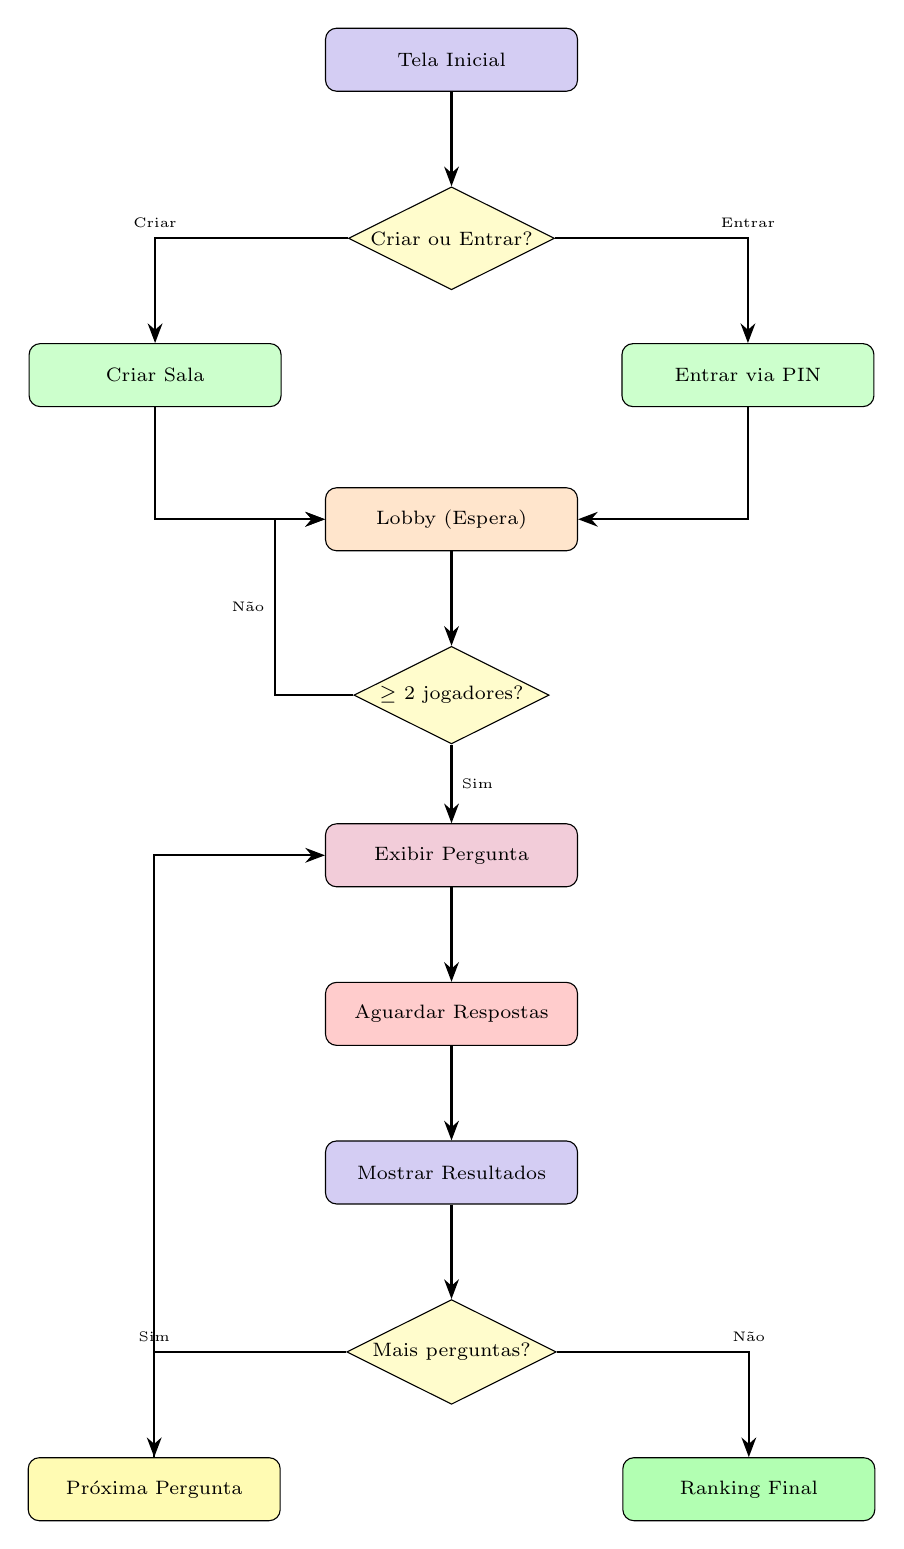
\begin{tikzpicture}[
  node distance=1.2cm,
  state/.style={rectangle, draw, rounded corners, minimum width=3.2cm, minimum height=0.8cm, text centered, font=\scriptsize, fill=#1},
  decision/.style={diamond, draw, aspect=2, minimum width=2cm, text centered, font=\scriptsize, fill=yellow!20, inner sep=1pt},
  arrow/.style={-{Stealth[length=2.5mm]}, thick},
]

\node[state=blue!20] (inicio) {Tela Inicial};
\node[decision, below=of inicio] (opcao) {Criar ou Entrar?};
\node[state=green!20, below left=1cm and 1.5cm of opcao] (criar) {Criar Sala};
\node[state=green!20, below right=1cm and 1.5cm of opcao] (entrar) {Entrar via PIN};
\node[state=orange!20, below=2.5cm of opcao] (lobby) {Lobby (Espera)};
\node[decision, below=of lobby] (minimo) {$\geq$ 2 jogadores?};
\node[state=purple!20, below=1cm of minimo] (pergunta) {Exibir Pergunta};
\node[state=red!20, below=of pergunta] (responder) {Aguardar Respostas};
\node[state=blue!20, below=of responder] (resultado) {Mostrar Resultados};
\node[decision, below=of resultado] (mais) {Mais perguntas?};
\node[state=yellow!30, below left=1cm and 1.5cm of mais] (proximo) {Próxima Pergunta};
\node[state=green!30, below right=1cm and 1.5cm of mais] (fim) {Ranking Final};

\draw[arrow] (inicio) -- (opcao);
\draw[arrow] (opcao) -| node[above, font=\tiny] {Criar} (criar);
\draw[arrow] (opcao) -| node[above, font=\tiny] {Entrar} (entrar);
\draw[arrow] (criar) |- (lobby);
\draw[arrow] (entrar) |- (lobby);
\draw[arrow] (lobby) -- (minimo);
\draw[arrow] (minimo) -- node[right, font=\tiny] {Sim} (pergunta);
\draw[arrow] (minimo.west) -- +(-1,0) |- node[left, font=\tiny, pos=0.25] {Não} (lobby.west);
\draw[arrow] (pergunta) -- (responder);
\draw[arrow] (responder) -- (resultado);
\draw[arrow] (resultado) -- (mais);
\draw[arrow] (mais) -| node[above, font=\tiny] {Sim} (proximo);
\draw[arrow] (proximo) |- (pergunta);
\draw[arrow] (mais) -| node[above, font=\tiny] {Não} (fim);

\end{tikzpicture}
\end{center}
\legend{Fonte: Elaborado pelo autor.}
\end{figure}

% ─── Apêndice C – Docker Compose ──────────────────────────────────────────
\chapter{Configuração Docker Compose}

O arquivo \texttt{docker-compose.yml} abaixo define a configuração completa para implantar a plataforma ExoGame em contêineres Docker, com restrições de recursos adequadas a um servidor de demonstração ou ambiente de avaliação acadêmica. O \textit{backend} é o \textbf{Phoenix/Elixir (BEAM)} --- escolhido por sua reconhecida superioridade em aplicações WebSocket de alta concorrência, conforme discutido na \autoref{sec:whatsapp} --- e o \textit{frontend} é o Next.js com saída \textit{standalone}.

\begin{lstlisting}[caption={docker-compose.yml -- orquestração dos serviços ExoGame (backend Phoenix/Elixir)},
                   label={lst:docker_compose}]
services:
  # Backend – Phoenix / Elixir (BEAM) ← backend principal
  backend:
    build:
      context: ./backend_elixir
      dockerfile: Dockerfile
    container_name: exogame_backend
    restart: unless-stopped
    environment:
      MIX_ENV: production
      PHX_SERVER: "true"
      PORT: "3001"
      PHX_HOST: "localhost"
      SECRET_KEY_BASE: "<gere com: mix phx.gen.secret>"
    ports:
      - "3001:3001"
    networks:
      - exogame_net
    deploy:
      resources:
        limits:
          cpus: "1.0"
          memory: 1024M
        reservations:
          cpus: "0.25"
          memory: 256M
    healthcheck:
      test: ["CMD","wget","--quiet","--tries=1","--spider",
             "http://localhost:3001/questions"]
      interval: 15s
      timeout: 5s
      retries: 5
      start_period: 30s

  # Frontend – Next.js (standalone)
  frontend:
    build:
      context: ./frontend
      dockerfile: Dockerfile
    container_name: exogame_frontend
    restart: unless-stopped
    environment:
      NODE_ENV: production
      NEXT_PUBLIC_BACKEND_URL: "http://localhost:3001"
      NEXT_PUBLIC_BACKEND_WS:  "ws://localhost:3001"
    ports:
      - "3000:3000"
    networks:
      - exogame_net
    depends_on:
      backend:
        condition: service_healthy
    deploy:
      resources:
        limits:
          cpus: "1.0"
          memory: 1024M
        reservations:
          cpus: "0.25"
          memory: 256M
    healthcheck:
      test: ["CMD","wget","--quiet","--tries=1","--spider",
             "http://localhost:3000"]
      interval: 15s
      timeout: 5s
      retries: 5
      start_period: 60s

networks:
  exogame_net:
    driver: bridge
\end{lstlisting}

Para iniciar a aplicação completa em ambiente Docker, basta executar:

\begin{lstlisting}[language={}]
docker compose up --build
\end{lstlisting}

O \textit{backend} estará disponível em \texttt{ainda a divulgar} e o \textit{frontend} em \texttt{ainda a divulgar}.
\end{apendicesenv}

% ----------------------------------------------------------
% Índice remissivo
% ----------------------------------------------------------
\phantompart
\printindex

\end{document}